\LARGE{ \textbf {Лекция №1} 12.02.2018 }\\
\Large Модели и методы анализа проектных решений

Литература :\\
Норенков И.П. Основы АП\\
САПР Модели технических объектов № 4\\
САПР Функциональное моделирование №5\\
Рябинький разностные схемы\\
Зенькевич Морган аппроксимации и К.Э.\\
bigor\\
wwwcdl.bmstu.ru --- Учебные материалы / математическое моделирование\\

\textbf {Блочно-иерархический подход к проектированию:} \\
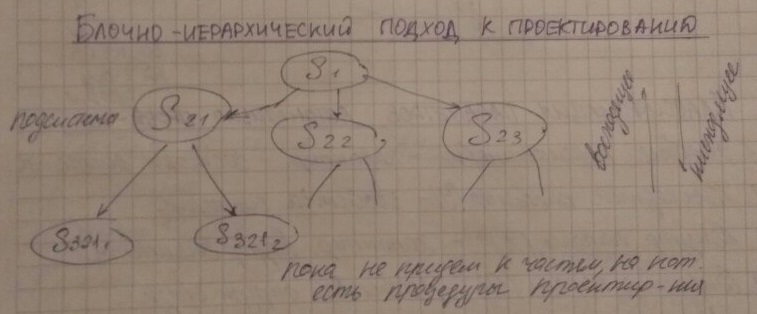
\includegraphics[width=\linewidth]{1}
\begin{center}
  Рисунок 1.\\
\end{center}
Разбиваем до тех пор, пока элементы не станут проектируемыми.\\
%$ S_1 - система S_{2i} - элемент $

\newpage

\textbf {Блок схема проектирования} \\
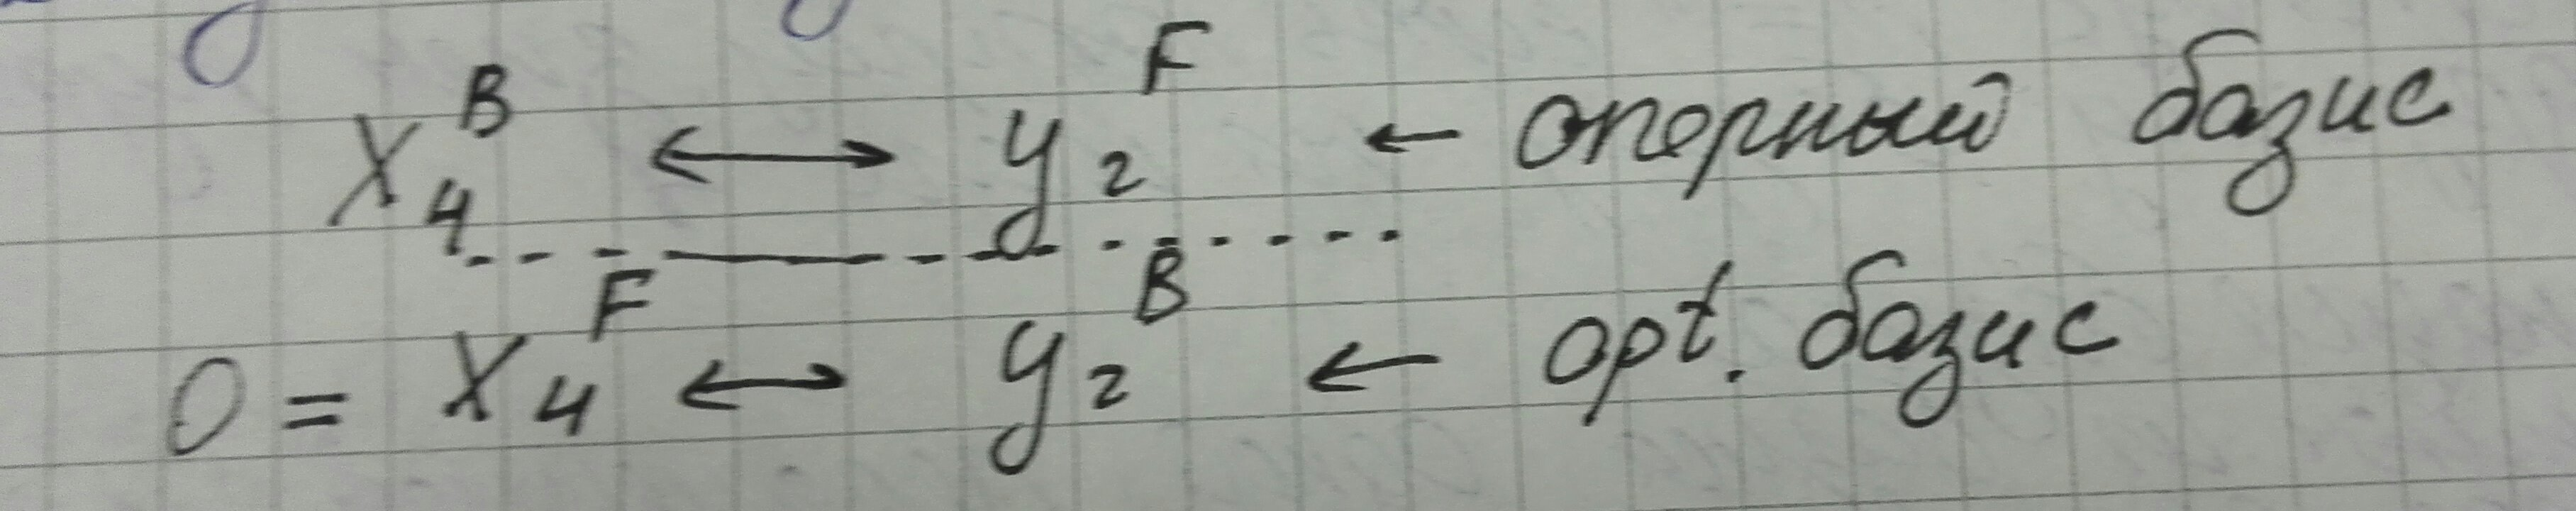
\includegraphics[width=\linewidth]{2}
\begin{center}
  Рисунок 2.\\
\end{center}

{\bfseries Классификация параметров при автоматизированном проектировании.}
\begin{itemize}
  \item  характеризующие состояние системы (фазовые переменные V)
  \item  характеризующие свойства системы (выходные параметры Y)
  \item  характеризующие свойства элементов (внутренние параметры X)
  \item  характеризующие свойства ОКР среды (внешние параметры Q)
\end{itemize}
{\itshape Математическая модель} — совокупность математических символов и связей между ними характеризующая важнейшие дляпроектировщика свойства реального объекта.\\
{\itshape Математическое моделирование} — процесс получения мат модели и оперирования ею с целью получения информации о свойствах реального объекта.\\

\textbf {Блок схема преобразования мат модели в процессе вычислений.} \\
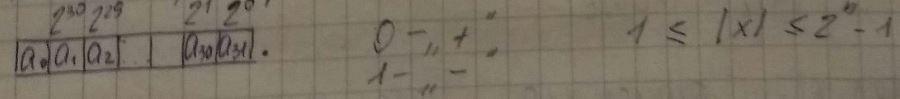
\includegraphics[width=\linewidth]{3}
\begin{center}
  Рисунок 3.\\
\end{center}

\newpage


\textbf {Методы решения СЛАУ:}\\
Точные
\begin{enumerate}
  \item Гаусса
  \item Численного разложения
\end{enumerate}
Итерационные
\begin{enumerate}
  \item Простой итерации
  \item Последовательно релаксации
  \item Метод сопряжённых градиентов
\end{enumerate}



Метод простой итерации
$$ A \cdot x + B = 0 $$
$$ x^{n+1} = A' \cdot x^n - B $$


\textbf { Методы решения нелинейных систем уравнений }\\
Метод Ньютона\\
\begin{flalign*}
  & F(x^*)=0, \quad \mbox {где $x^*$ - точное решение} \\
  & x^* = x + \Delta x\\
  & F(x + \Delta x)= F(x) + \frac{ \partial F(x)}{\partial x} \cdot \Delta x + \cdots = 0 \\
  \end{flalign*}
  \begin{equation}
    g(x) \cdot \Delta x =  -F(x) ,
 \end{equation}
где $F(x)$ - вектор невязок , $g(x)$ - матрица Якоби  , $\Delta x$ - вектор поправок\\
 \begin{flalign*}
  & g(x) = \frac{ \partial F(x)}{\partial x} \\
  &x^{n+1}= x^n + \Delta x \\
  & \mbox {Подставляем последнее уравнение в уравнение (1)}
\end{flalign*}
